\documentclass{beamer}


\usepackage[spanish]{babel} 
\usepackage[utf8]{inputenc} 
\usepackage{amsmath}
\usepackage{hyperref}
\usepackage[nodayofweek]{datetime}
\usepackage{pgfpages}

\usepackage{caption}
\usepackage{subcaption}


\makeatletter
\def\verbatim@font{\ttfamily\tiny}
\makeatother

%~ \usetheme{Berkeley}
%~ \usetheme{CambridgeUS} %~ Ok 3
%~ \usetheme{Boadilla} %~ Ok 2
\usetheme{boxes} %~ Ok 1
\setbeamerfont{frametitle}{size=\small}

\usecolortheme{seahorse} %~ OK
%~ \usecolortheme{dolphin} 
%~ \usecolortheme{beaver}
%~ \usecolortheme{whale}
%~ \usecolortheme{lily}


%~ \usetheme{Frankfurt}
%~ \usetheme{Madrid}
%~ \usetheme{Malmoe}

%~ \setbeamercovered{transparent}

\logo{%
	   
\includegraphics[scale=.25]{img/logoIBR2016_byn.png}
   }
\title[]{Estudios sobre la regulación de la expresión génica por microARNs en plantas mediante estrategias bioinformáticas}

\author{Uciel Chorostecki}
\institute[IBR]{ \\Director Dr. Javier Palatnik\\Instituto Biología Molecular y Celular Rosario}
\date{}

\begin{document}

\frame{\titlepage}

\section{Introducción}

\begin{frame}{miARNs}
    \begin{itemize}
        \item Los microARNs (miARNs) son ARN pequeños de 20-22 nt que regulan la expresión génica en animales y plantas. 
        \item En plantas controlan procesos vitales como el desarrollo, señalización hormonal y respuestas al estrés
    \end{itemize}
\end{frame}

\section{Objetivos}

\begin{frame}{Objetivos}
    \setbeamercovered{transparent=25}
	\begin{enumerate}[<+->]
        \item Identificar genes regulados por miARNs en plantas.
        \item Estudiar la biogénesis de los miARNs en plantas.
	\end{enumerate}
\end{frame}

\begin{frame}{Objetivos específicos}
    \setbeamercovered{transparent=25}
		\pause
		\begin{itemize}
            \item<-2> Diseñar una estrategia y una herramienta web para la identificación de genes blancos regulados por miARNs en plantas.
			\item<-1> Desarrollar herramientas para el análisis de los intermediarios de procesamiento de miARNs en plantas.
			\item<-1> Identificar y caracterizar precursores de miARNs en distintas especies que tengan mecanismos de procesamiento distintos.
			\item<-1> Caracterizar la relación entre la evolución de los precursores de miARNs en plantas y los mecanismos de procesamiento determinados previamente.
        \end{itemize}
\end{frame}


\section{Resultados}

\subsection{Resultados 1}

\begin{frame}{Aplicaciones bioinformáticas para el estudio de interacciones miARN-gen blanco}
\end{frame}

\begin{frame}{Conservación y divergencia de miARNs en distintas especies}
	\begin{center}
		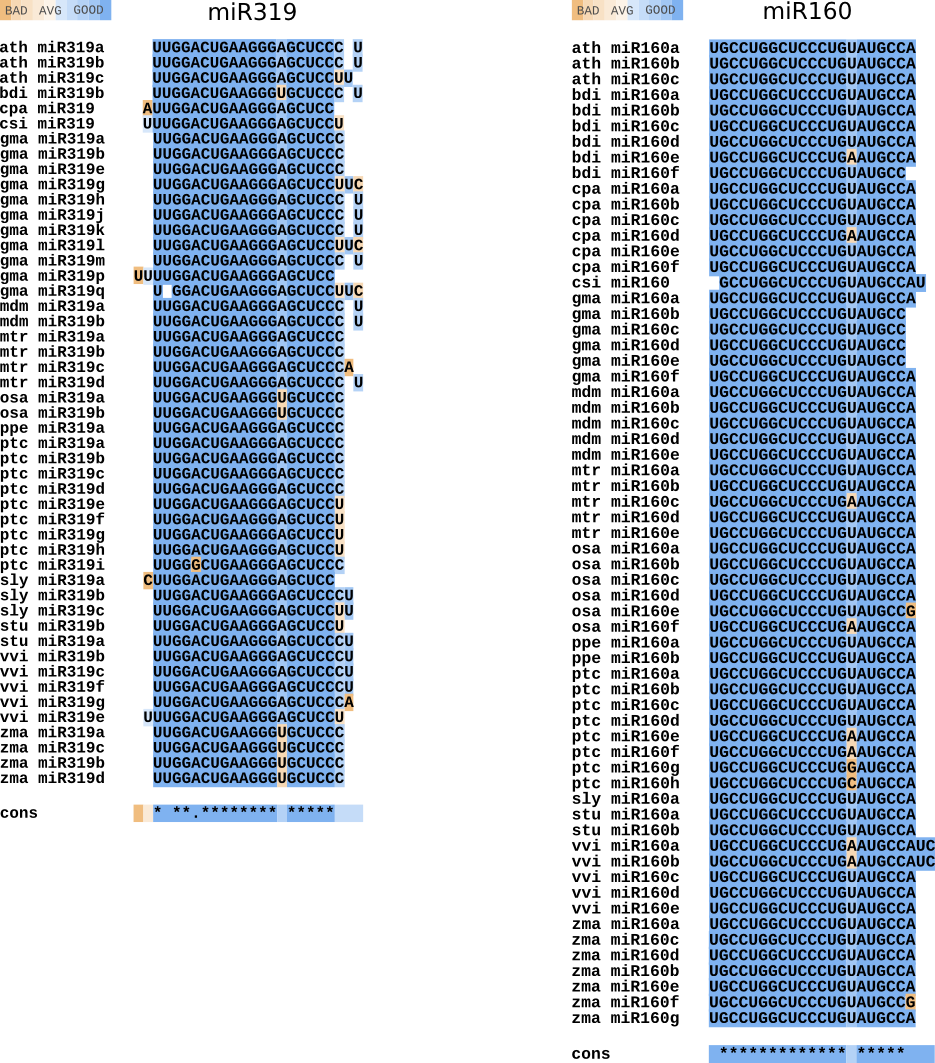
\includegraphics[width=0.5\textwidth]{img/variabilidad_maduro.png}
	\end{center}
\end{frame}

\begin{frame}{22 miARNs que están conservados en Angiospermas}
	\begin{center}
		
\includegraphics[width=0.5\textwidth]{img/NAR_fig1_01.png}
	\end{center}
\end{frame}

\begin{frame}{Secuencias consensos de 18 nt (2-19)}
	\begin{center}
		
\includegraphics[width=0.5\textwidth]{img/NAR_fig1_02.png}
	\end{center}
\end{frame}

\begin{frame}{Primera búsqueda general de potenciales genes blancos}
	\begin{center}
		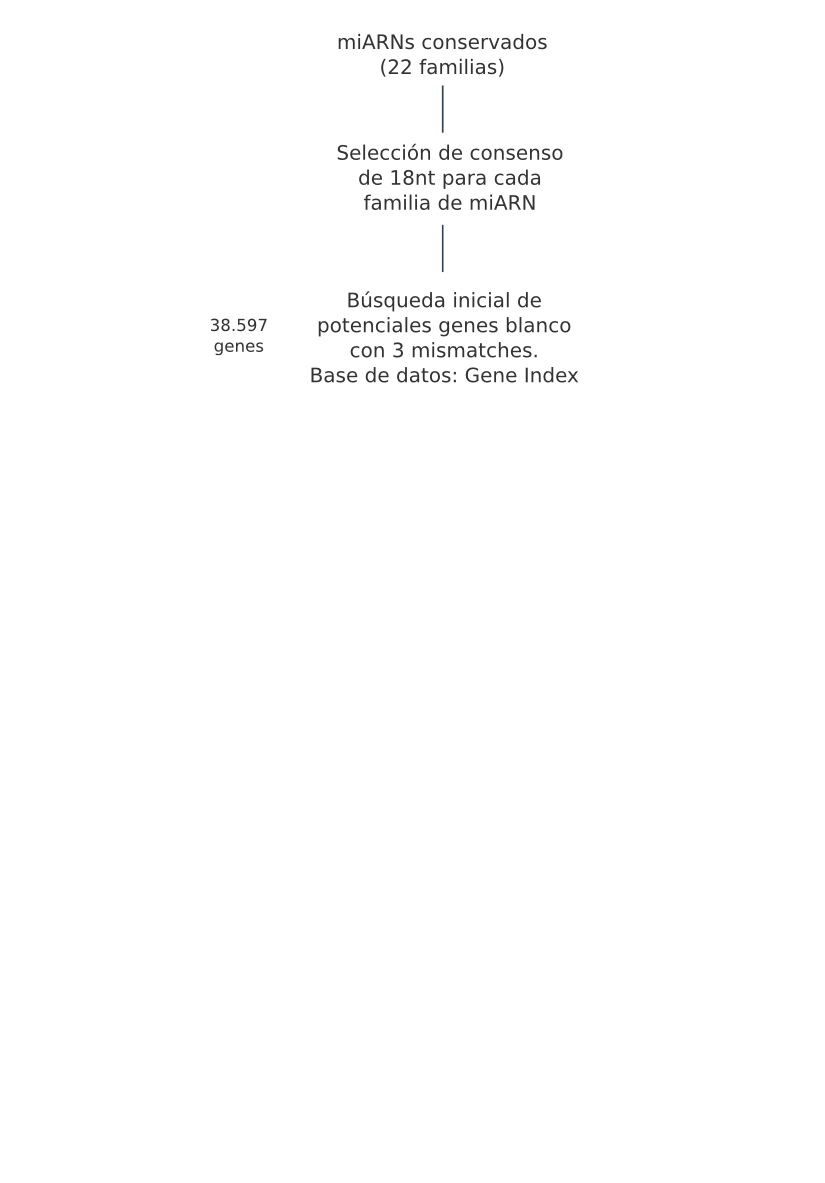
\includegraphics[width=0.5\textwidth]{img/NAR_fig1_03.png}
	\end{center}
\end{frame}

\begin{frame}{Filtros de evolución y empíricos de interacción miARN-gen blanco}
	\begin{center}
		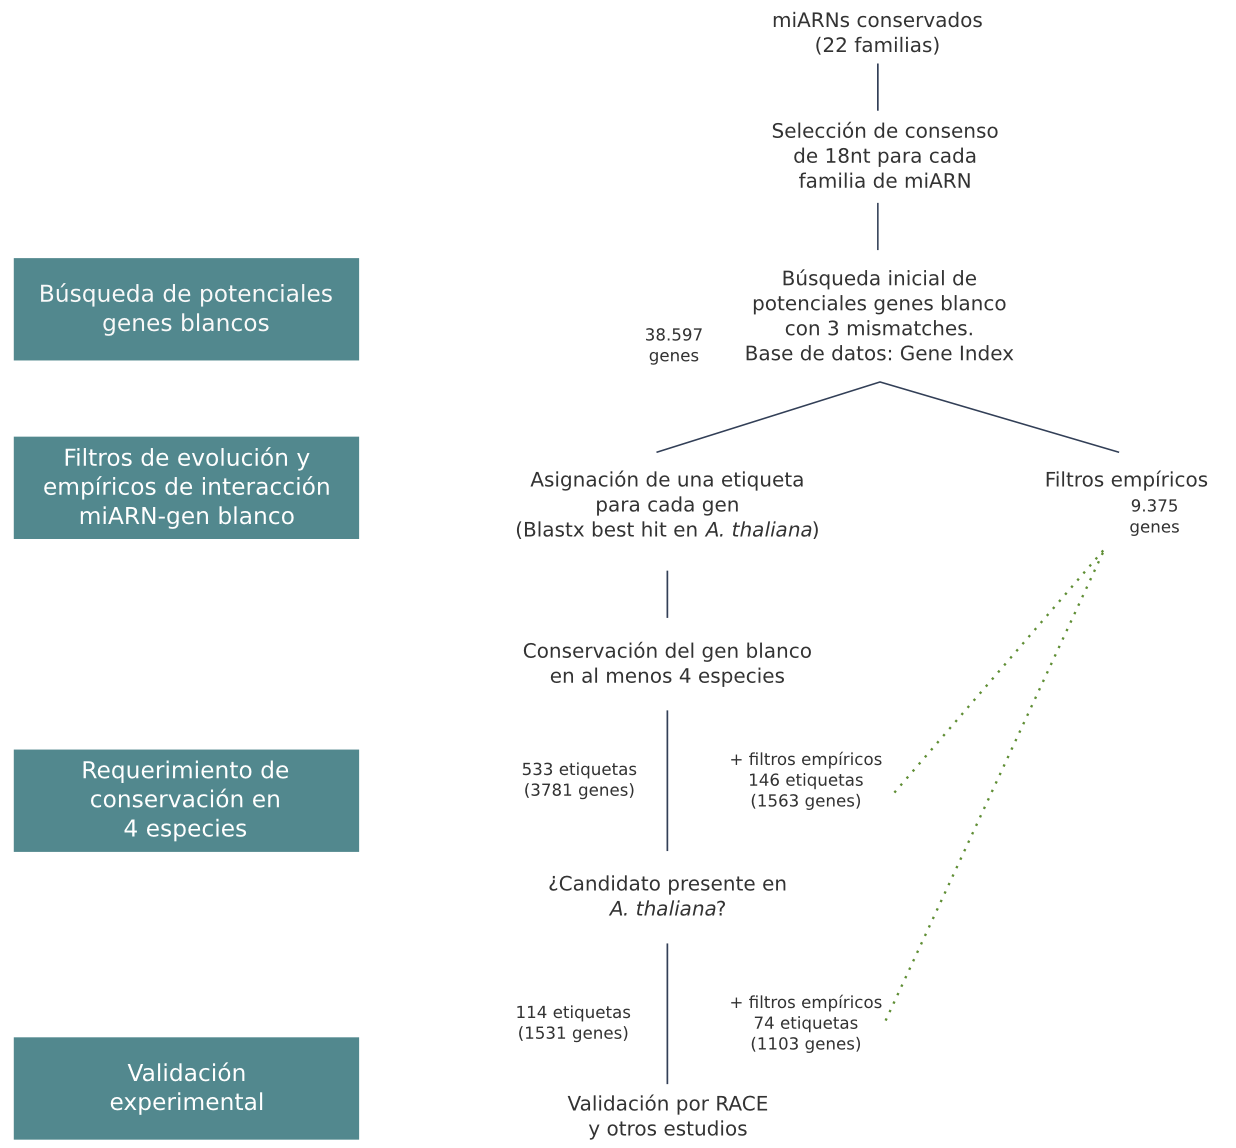
\includegraphics[width=0.5\textwidth]{img/NAR_fig1_04.png}
	\end{center}
\end{frame}

\begin{frame}{Mínimo de 4 especies requeridas}
	\begin{center}
		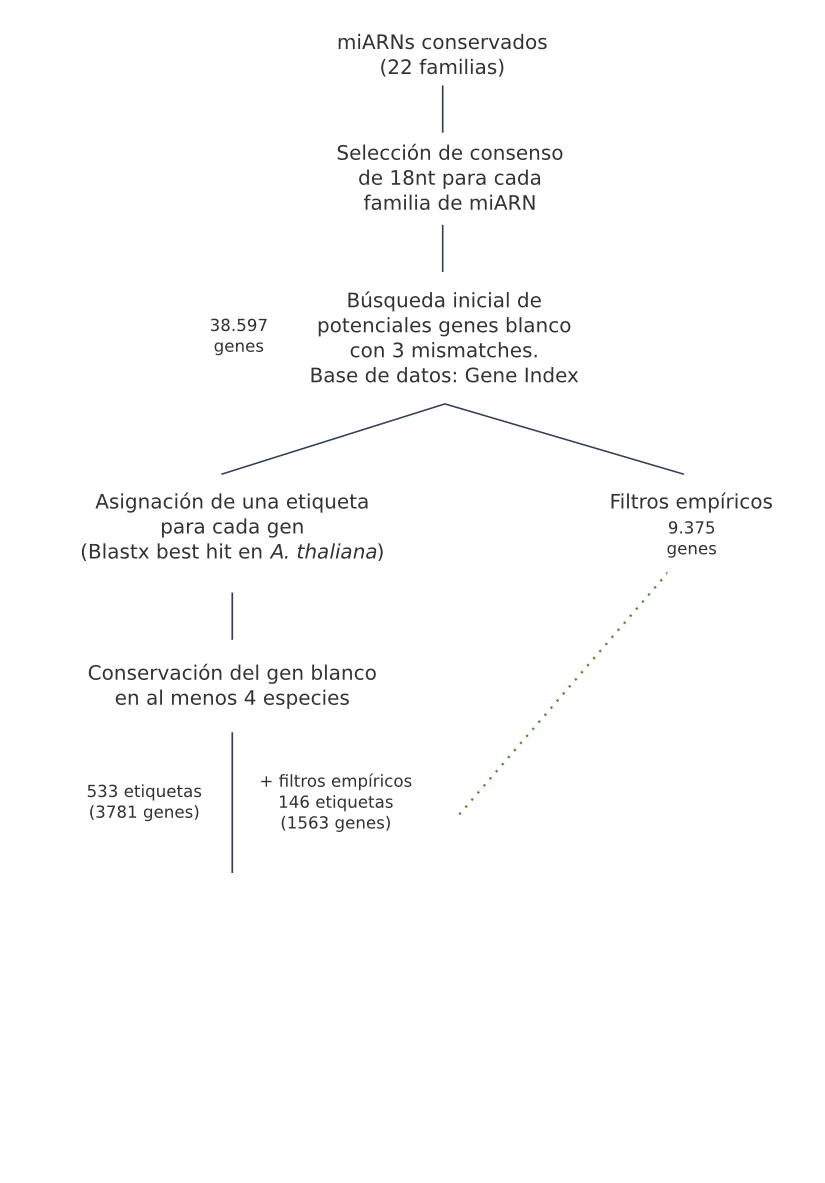
\includegraphics[width=0.5\textwidth]{img/NAR_fig1_05.png}
	\end{center}
\end{frame}

\begin{frame}{Genes blanco en \textit{A. thaliana}}
	\begin{center}
		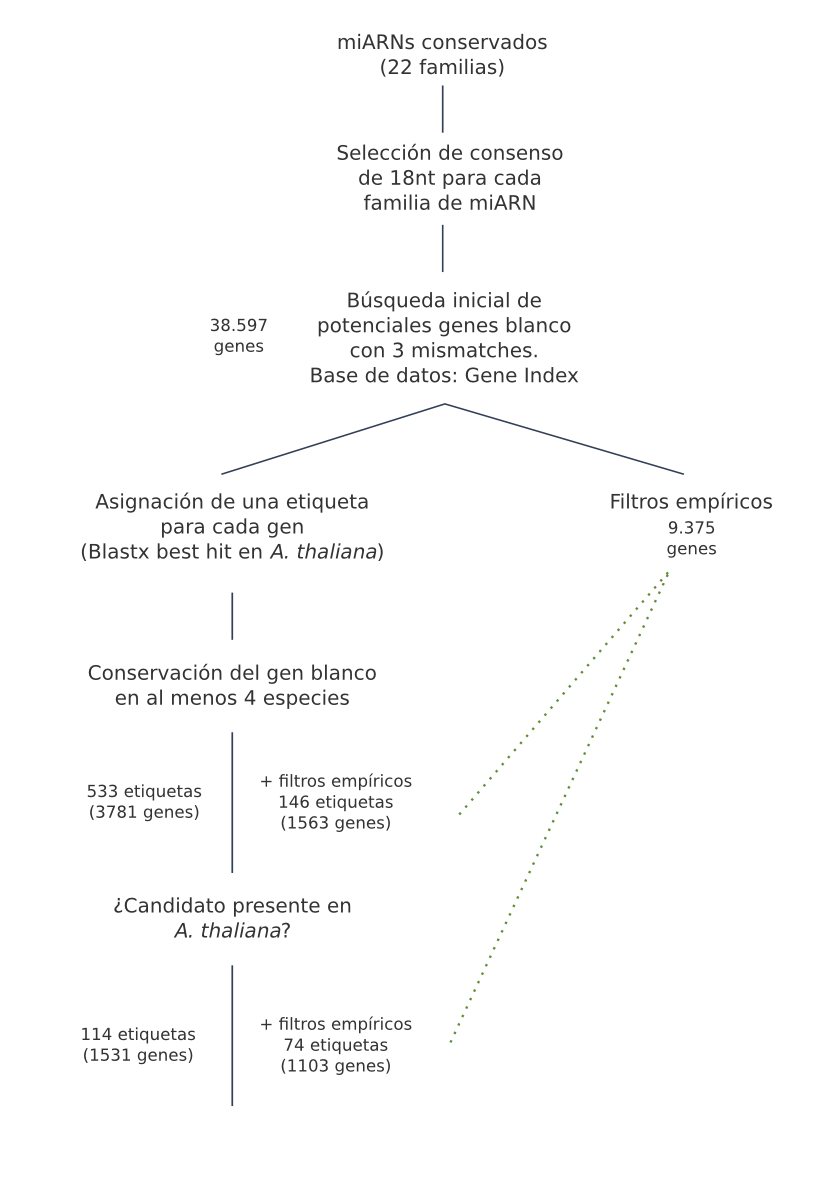
\includegraphics[width=0.5\textwidth]{img/NAR_fig1_06.png}
	\end{center}
\end{frame}

\begin{frame}{Validación experimental}
	\begin{center}
		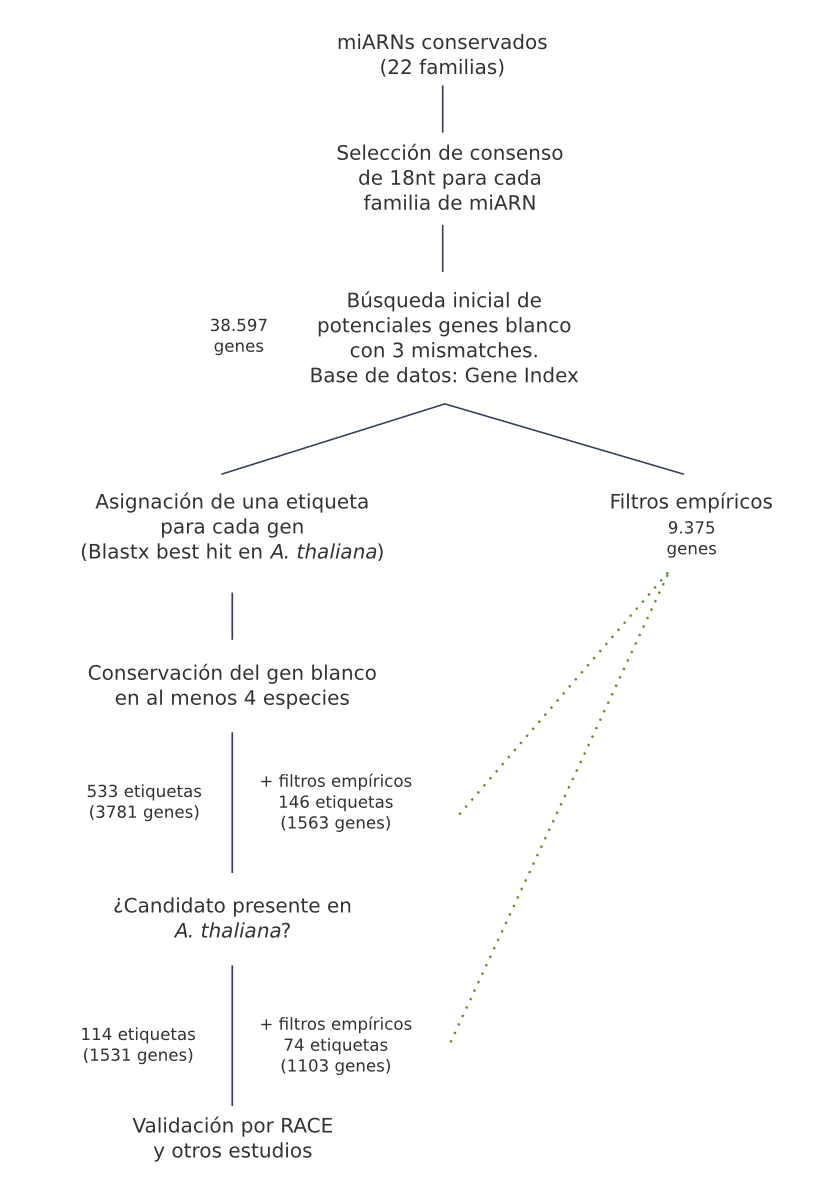
\includegraphics[width=0.5\textwidth]{img/NAR_fig1_07.png}
	\end{center}
\end{frame}

\begin{frame}{xxxx}
	\begin{center}
		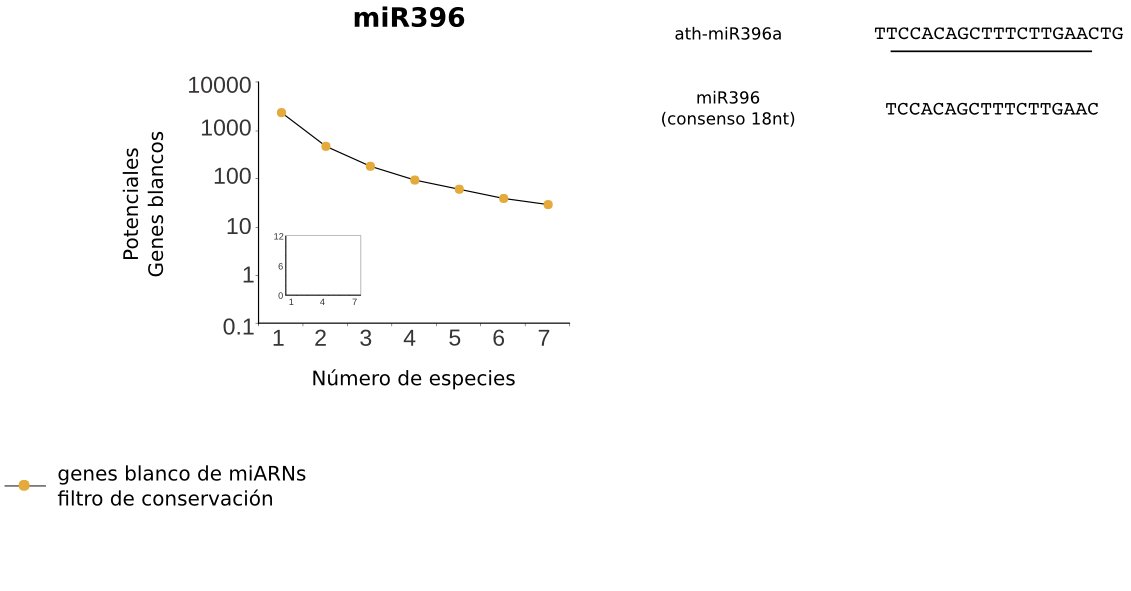
\includegraphics[width=0.5\textwidth]{img/NAR_fig2_01.png}
	\end{center}
\end{frame}

\begin{frame}{xxxx}
	\begin{center}
		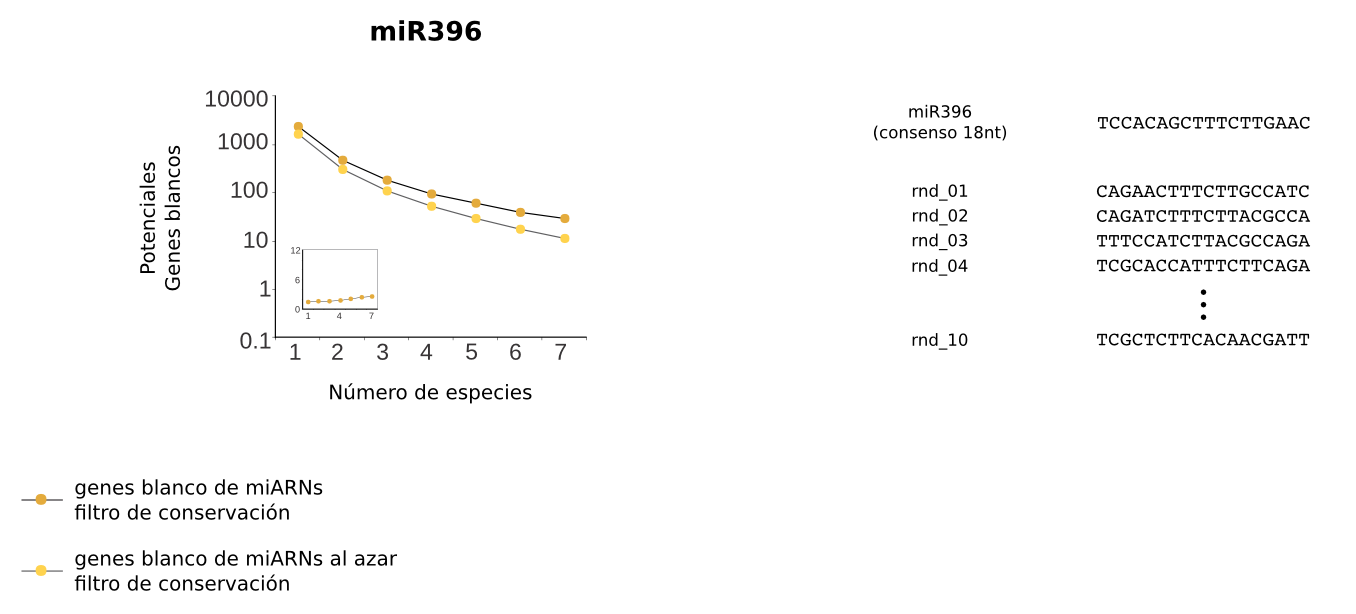
\includegraphics[width=0.5\textwidth]{img/NAR_fig2_02.png}
	\end{center}
\end{frame}

\begin{frame}{xxxx}
	\begin{center}
		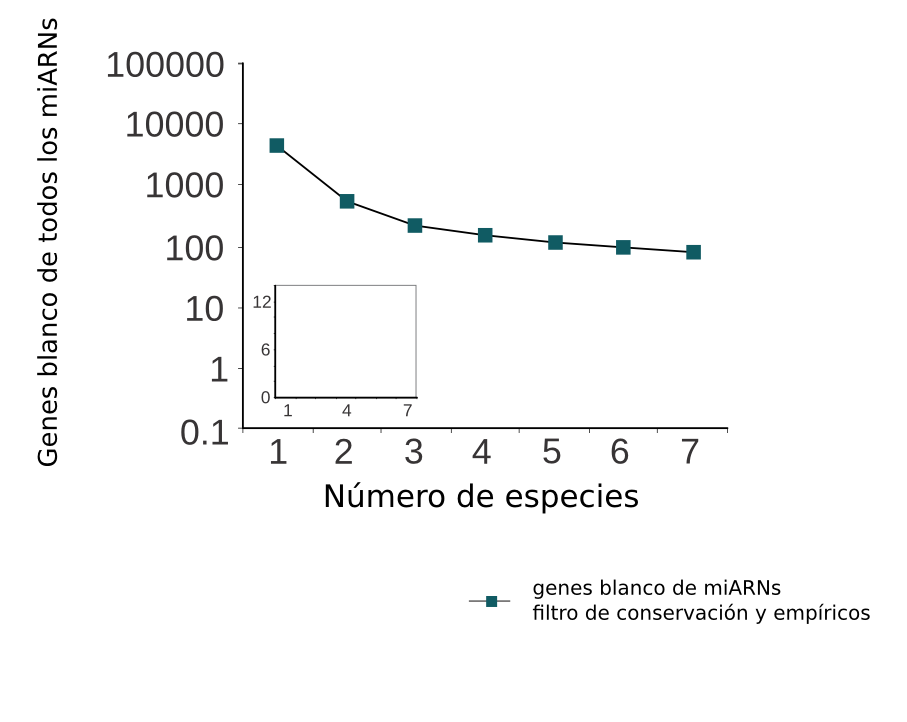
\includegraphics[width=0.5\textwidth]{img/NAR_fig2_03.png}
	\end{center}
\end{frame}

\begin{frame}{xxxx}
	\begin{center}
		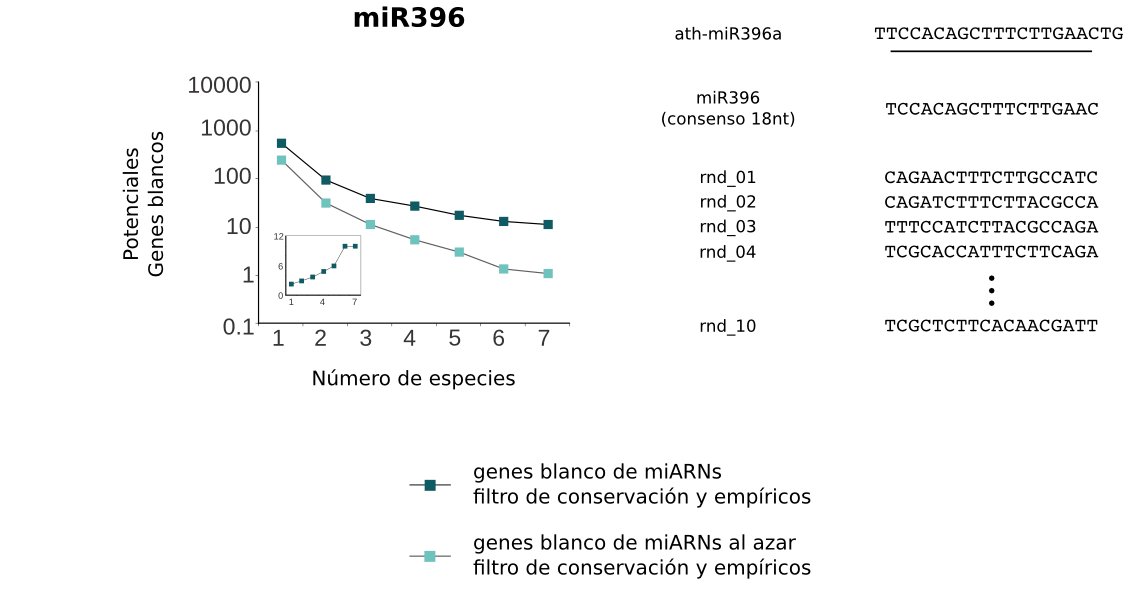
\includegraphics[width=0.5\textwidth]{img/NAR_fig2_04.png}
	\end{center}
\end{frame}

\begin{frame}{xxxx}
	\begin{center}
		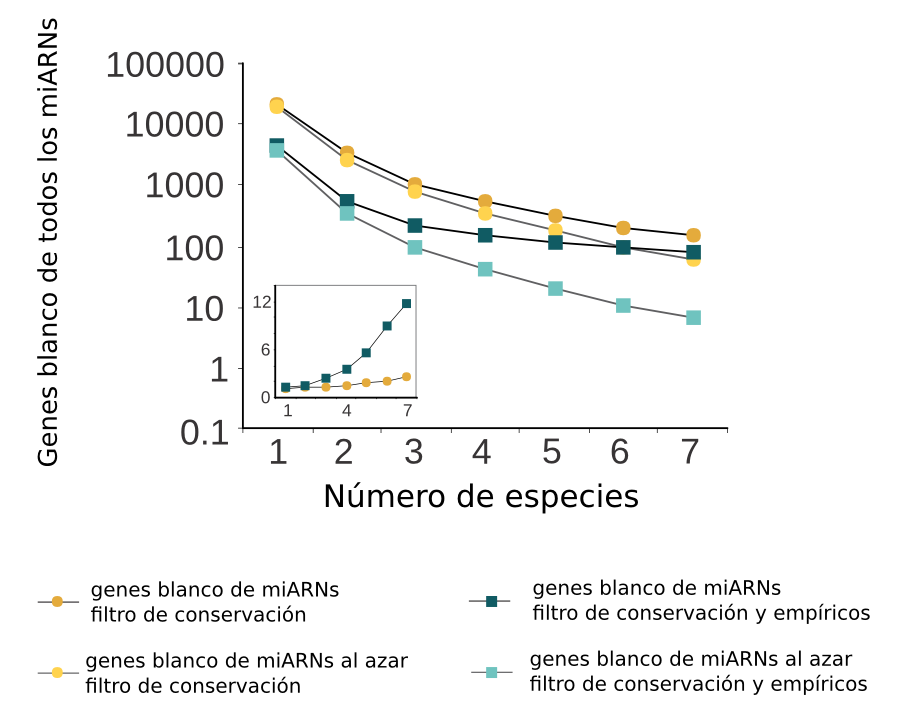
\includegraphics[width=0.5\textwidth]{img/NAR_fig2_05.png}
	\end{center}
\end{frame}

\begin{frame}{xxxx}
	\begin{center}
		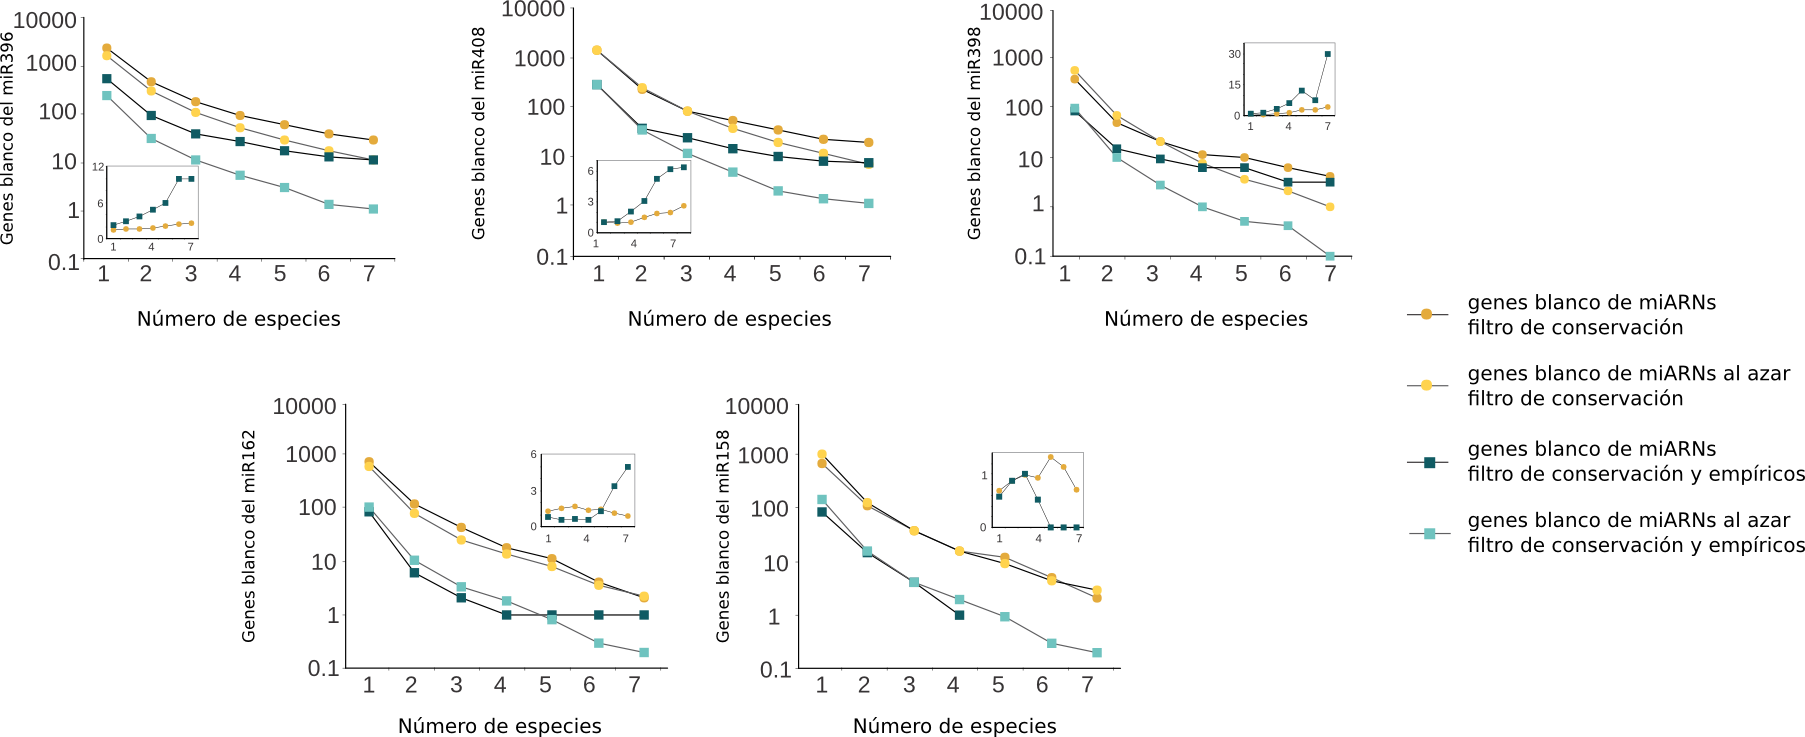
\includegraphics[width=1\textwidth]{img/NAR_fig2_bis.png}
	\end{center}
\end{frame}


\subsection{Resultados 2}

\subsection{Resultados 3}


\section{Conclusiones}


\begin{frame}{Conclusión I}
	\begin{center}
		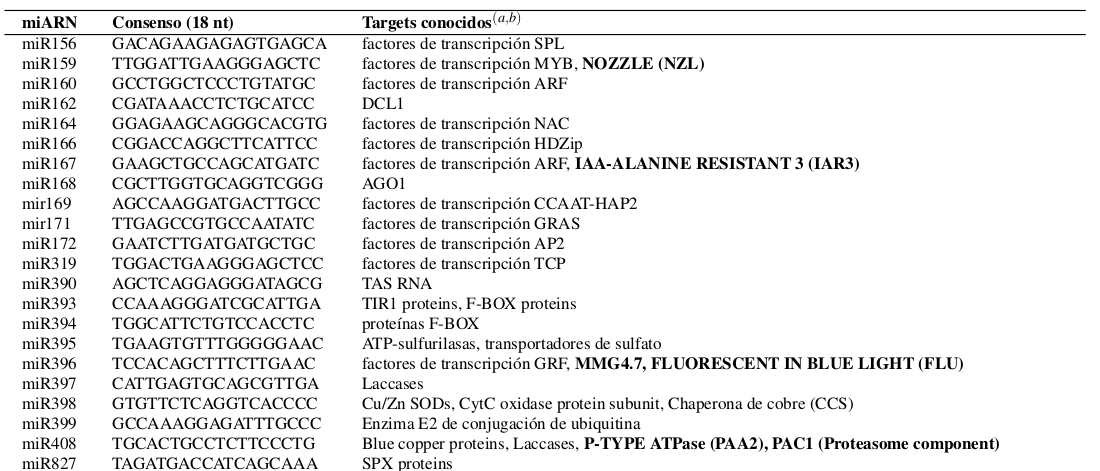
\includegraphics[width=.8\textwidth]{img/miRNAs_y_genes_blancos.png}
	\end{center}
\end{frame}

\begin{frame}{Conclusión I}
	\begin{itemize}
        \item<1-> a
        \item<2-> a
        %~ \vspace{1cm}
        \item<3-> a
	\end{itemize}
\end{frame}



\begin{frame}{}
	\begin{center}
		\Huge Muchas gracias.
	\end{center}
\end{frame}

\end{document}
